\chapter{Material und Methoden}
\label{kap:material_und_methoden}

\section{Material}
\label{sec:material}

\subsection{Chemikalien}
\label{subsec:chemikalien}

\begin{table}[H]
	\centering
	\keepXColumns
	\caption{Auflistung der verwendeten Chemikalien.}
	\begin{tabularx}{\textwidth}{X X}
		\textbf{Bezeichnung}	&	\textbf{Bezogen von}	\\
		\toprule
		\toprule
		\ac{EDC}	&	Sigma Aldrich	\\
		&\\
		\ac{NHS}	&	Sigma Aldrich	\\
		&\\
		\ac{CMA}	&	Santa Cruz Biotechnologie	\\
		&\\
		\ac{PBS}	&	Biochrom	\\
		&\\
		Ethanol 99\% unvergällt	&	Carl Roth	\\
		&\\
		\ac{HCl} (32 \%)	&	Carl Roth	\\
		&\\
		\ac{NaOH}	&	Carl Roth	\\
		&\\
		Allylamin	&	Sigma Aldrich	\\
		&\\
		Vitamin E	&	Sigma Aldrich	\\
		\toprule
		\toprule
	\end{tabularx}
	\label{tab:chemikalien}
\end{table}

Alle Chemikalien wurden vor der Verwendung, falls nicht anders vermerkt, nicht weiter bearbeitet. \acs*{CMA} steht bei Santa Cruz Biotechnology seit Juli 2017 nicht mehr im Sortiment.

\subsection{Substrate}
\label{subsec:substrate}

\begin{table}[H]
	\centering
	\keepXColumns
	\captionabove{Auflistung der verwendeten Substrate.}
	\begin{tabularx}{\textwidth}{X X}		
		\textbf{Bezeichnung}	&	\textbf{Bezogen von}	\\
		\toprule
		\toprule
		GE Window DLC-Substrates	&	UQG Optics	\\
		&\\
		NPG-10 Cantilever mit HDC Spitzen	&	Bruker/ Nanotools	\\
		\toprule
		\toprule
	\end{tabularx}
	\label{tab:substrate}
\end{table}

Das GE-Window ist ein drei mm dickes Germanium-Glass-Substrat, beschichtet mit sieben µm \ac{DLC}. Die NPG-10 Cantilever von Bruker wurden von Nanotools mit einer \ac{HDC} Spitze modifiziert.

\subsection{Geräte und Software}
\label{subsec:geräte_und_software}

\begin{table}[H]
	\centering
	\keepXColumns
	\captionabove{Auflistung von verwendeten Geräten und verwendeter Software.}
	\begin{tabularx}{\textwidth}{X X}
		\textbf{Bezeichnung}	&	\textbf{Hersteller}	\\
		\toprule
		\toprule
		Nanowizard I\textsuperscript{\textregistered}	&	JPK Instruments AG	\\
		&\\
		UV Penray ($\lambda = 254~nm$)	&	UVP, LLC	\\
		&\\
		MATLAB	&	Mathworks	\\
		\toprule
		\toprule
	\end{tabularx}
	\label{tab:geräte_software}
\end{table}

\section{Methoden}
\label{sec:methoden}

\subsection{Oberflächenfunktionalisierung der Substrate}
\label{subsec:oberflächenfunktionalisierung_der_substrate}

Bei der gesamten Handhabung der \spitzen~war auf einen adäquaten Schutz vor elektrostatischer Entladung zu achten. Aus diesem Grund wurde mit den \spitzen~auf einer Schutzmatte gegen Elektrostatische Entladung gearbeitet. Zur persönlichen Schutzausrüstung gehörte zusätzlich ein Erdungsarmband. Um Beschädigung des Cantilevers zu vermeiden, wurde der gesamte $Si_3N_4$-Chip seitlich um 90° verkippt durch Flüssigkeitsgrenzflächen geführt. Bevor eine Funktionalisierung gestartet werden konnte, wurden \spitzen~und Substrate von organischen Verunreinigungen befreit. Die \spitzen~wurden dazu 90 min mit einer UV-Lampe beleuchtet, während die Substrate für diese Zeit in einer 5\% Hellmannex-Lösung im Ultraschallbad behandelt wurden. Die Substrate wurden anschließend für weitere 10 min mit doppelt destilliertem Wasser im Ultraschallbad gespült. Um die \spitzen~und Subrate mit terminalen \aminos~zu modifizieren wurde folgendes Protokoll verwendet:

\subsubsection{Präparation der Funktionalisierungslösungen}
\label{subsubsec:präparation_der_funktionalisierungslösungen}

\spitzen~und Substrate wurden in getrennten Glasgefäßen (ca. 3 ml Volumen) funktionalisiert. Die Ansätze beider Gefäße setzten sich jeweils aus ca. 2,7 ml reinem Ethanol (eingefüllt \textit{via} Tropfpipette) und ca. 0,3 ml Allylamin (eingefüllt \textit{via} 1 ml Spritze mit Kanüle des Durchmessers 0,9 mm) zusammen. Nach dem Vorlegen von Allylamin wurde anschließend Ethanol hinzugegeben. Der Ansatz wurde durch dreimaliges \enquote{auf und ab pipettieren} mit der Tropfpipette durchmischt.

\subsubsection{Oberflächenfunktionalisierung}
\label{subsubse:oberflächenfunktionalisierung}

Gereinigte \spitzen~und Substrate wurden in jeweils ein Gefäß mit einem Funktionalisierungsansatz gegeben. Zum Starten der Oberflächenfunktionalisierung, wurden beide Ansätze in eine UV-Kammer gegeben und unter Stickstoffbegasung mit einer UV-Lampe ($\lambda = 254~nm$) über eine Zeit von 3 Stunden bestrahlt.

\subsubsection{Stoppen der Funktionalisierung}
\label{subsubsec:stoppen_der_oberflächenfunktionalisierung}

Die Oberflächenfunktionalisierung wurde in einer Vitamin-E Lösung gestoppt, wobei das Vitamin-E als Radikalfänger diente. Zur Herstellung der Vitamin-E Lösung wurde in eine Petrischale, gefüllt mit reinem Ethanol, eine Spatelspitze Vitamin-E durch Rühren gelöst. Zum Stoppen der Funktionalisierung wurden \spitzen~und Substrate für zwei Minuten in die Lösung gegeben und anschließend in ein zweites Gefäß mit reinem Ethanol überführt.

\subsubsection{Entfernen nicht gebundener Reaktanden}
\label{subsubsec:entfernen_nicht_gebundener_reaktanden}

Um ungebundenes Allylamin von den Oberflächen der \spitzen~und Substrate zu entfernen, wurden \spitzen~und Substrate getrennt voneinander gereinigt. Die Substrate wurden in ein Becherglas, gefüllt mit einer 1:2 Verdünnung aus reinem Ethanol und doppelt destilliertem Wasser, gegeben und für insgesamt 40 Minuten in einem Ultraschallbad gereinigt. Die \spitzen~ruhten in dieser Zeit in reinem Ethanol. Substrate, sowie \spitzen~wurden anschließend für ca. 5 Minuten an Luft getrocknet. Zur Lagerung wurden \spitzen~und Substrate in einen Exsikkator mit Trocknungsmittel (Silicagel) gegeben.

\subsection{Vorbereitung der Versuche}
\label{subsec:vorbereitung_der_versuche}

\subsubsection{Präparation der Kopplungslösungen}
\label{subsubsec:präparation_der_kopplungslösungen}

Zunächst wurde eine \ac{CMA}-Lösung hergestellt. Dazu wurden 1 mg \ac{CMA} mit 0,1 ml \ac{PBS} mit einem pH-Wert von 6,5 (der pH-Wert wurde mit 32 \% \ac{HCl} eingestellt) gelöst. Dazu wurde der Ansatz in ein 1,5 ml Zentrifugenröhrchen gegeben und auf einem Vortexer für 20 min fixiert.\\
Anschließend wurde eine \ac{EDC}/ \ac{NHS}-Lösung hergestellt. Dazu wurden 10 mg \ac{NHS} und 25 mg \ac{EDC} in einem 1,5 ml Zentrifugenröhrchen, in 0,5 ml derselben \ac{PBS}-Lösung wie oben, auf einem Vortexer für ca. 10 Sekunden gemischt.\\
Zur Herstellung der Kopplungslösung wurden 0,1 ml der \ac{EDC}/ \ac{NHS}-Lösung mit 0,1 ml der \ac{CMA}-Lösung gemischt, sodass die \ac{CMA}-Konzentration bei ca. 5 mg/ml lag.

\subsubsection{Kopplung der Spacer an die Substrate}
\label{subsubsec:kopplung_der_spacer_an_die_substrate}

Die Kopplung von \spacer~mit dem Substrat bzw. \spitze~geschah durch nachfolgende Sequenz:

\begin{enumerate}
	\renewcommand\labelenumi{\bfseries\theenumi.}
	
	\item Beschichten des Substrates mit 30 \% Essigsäure \textit{via} Tropfpipette für 3 min.
	\item Entfernen der Essigsäure durch abpipettieren \textit{via} Tropfpipette und Zugabe von ca. 50~µl der Kopplungslösung für 10 min.
	\item Entfernen der Kopplungslösung durch dreifaches Spülen mit jeweils 1~ml der \ac{PBS}-Lösung aus dem vorherigen Abschnitt.
	\item Hinzufügen von ca. 50 µl der \ac{EDC}/ \ac{NHS}-Lösung aus dem vorherigen Abschnitt,  für 3 min.
	\item Auffüllen der Petrischale mit \ac{PBS} des gewünschten pH-Wertes\footnote{Die pH-Werte wurden mit einer 1M NaOH-Lösung oder mit 32\% \ac{HCl} eingestellt.} bis die Oberfläche des Substrates ca. 2 bis 5 mm unterhalb des Flüssigkeitsmeniskus lag.
	
\end{enumerate}

Anschließend wurden die Messungen am \ac{AFM} gestartet.

\subsection{Durchführung der Versuche}
\label{subsec:durchführung_der_versuche}

Die Durchführung aller Versuche gliederte sich in drei Abschnitte:

\begin{enumerate}
	\renewcommand\labelenumi{\bfseries\theenumi.}
	
	\item Kalibrierung des Cantilevers
	\item Auswahl der x,y-Position auf dem Substrat 
	\item Start des Force-Clamp-Experiments
	
\end{enumerate}

\subsubsection{Kalibrierung des Cantilevers}
\label{subsubsec:kalibrierung_des_cantilevers}

Die Kalibrierung des Cantilevers diente der Umrechnung der Cantileverauslenkung von Einheiten der Spannung in Einheiten der Kraft. Die Kalibrierung erfolgte in zwei Schritten. Zunächst wurde die optische Sensitivität des Cantilevers ermittelt. Dies diente der Umrechnung des Spannungssignals an der Photodiode in die Auslenkung des Cantilevers in Einheiten der Länge. Anschließend wurde die Federkonstante des Cantilevers über die Methode des thermischen Rauschens bestimmt \cite{Butt.1995}. Über die Federkonstante wurde die Cantileverauslenkung in Einheiten der Kraft umgerechnet. Eine detaillierte Anleitung des Ablaufs kann in der Arbeit von T.Becke \textit{et al.} \cite{Becke.2018} nachgeschlagen werden.\\
Nach der Kalibrierung mussten die Regelparameter des \acp{AFM} (Integralwert und Proportionalwert) an das System angepasst werden.

\subsubsection{Auswahl der x,y-Position des Force-Clamp-Experiments auf dem Substrat}
\label{subsubsec:auswahl_der_x_y_position_des_force_clamp_experiments_auf_dem_substrat}

Zunächst wurden die \spitzen~mittels einer Topview-Kamera auf die Mitte des Substrats ausgerichtet. Um zu verifizieren, ob an dieser Stelle Einzelmolekülinteraktionen zwischen \spitze~bzw. Substrat und \spacer~auftraten, wurde zuerst ein Force-Ramp-Experiment durchgeführt. Falls keine entsprechenden Interaktionen zu beobachten waren, wurde der Cantilever auf eine andere Stelle des Substrats ausgerichtet. Da die \ester~in Lösung nicht unbegrenzt stabil waren \cite{Hayworth}, wurde die Verifizierung der Position in maximal 30 min durchgeführt. Dazu wurde mittels der \ac{AFM}-Software ein quadratisches Raster mit einer Kantenlänge von $100~\mu m$ und 5 Messpunkte pro Achse (insgesamt 25 Messpunkte) programmiert und abgefahren. Details der Force-Ramp-Experimente können der Tabelle~\ref{tab:force-ramp-parameter} entnommen werden. Eine ausführliche Beschreibung der Force-Ramp-Experimente erfolgte in Abschnitt~\ref{subsec:kraftkurven}

\subsubsection{Start des Force-Clamp-Experiments}
\label{subsubsec:start des force-clamp-experiments}

Nachdem Auswählen einer passenden Stelle auf dem Substrat, wurde das Force-Clamp-Experiment durchgeführt. Um möglichst viele Einzelmolekülinteraktionen zu messen, wurden die Messpunkte des vorherigen Rasters auf 10 pro Achse (insgesamt 100 Messpunkte) erhöht. Jeder Messpunkt wurde zudem dreimal angefahren. Damit erhöhte sich die Messdauer auf 2,5 Stunden. Eine Anpassung der Parameter für verschiedene Experimente war nur im 3. Segment nötig. Hier wurde die Länge des Initial Retract für jedes Paar aus \spitze~und Substrat während des Experiments neu bestimmt. Die Länge schwankte dabei von $100$ bis $500~nm$. Details der Force-Clamp-Experimente können aus Tabelle~\ref{tab:force-clamp-parameter} entnommen werden. Eine ausführliche Beschreibung der Force-Clamp-Experimente erfolgte in Abschnitt~\ref{subsec:kraftkurven}.


\begin{table}[H]
	\centering
	\keepXColumns
	\captionabove{Experimenteller Ablauf der Force-Ramp-Experimente.}
	\begin{tabularx}{\textwidth}{X X X X}
		\multicolumn{2}{l}{\textbf{Parameter}}	&	\textbf{Einheit}	&	\textbf{Wert}	\\
		\toprule
		\toprule
		\multicolumn{4}{c}{Scanbereich}	\\
		\toprule
		\multicolumn{2}{l}{Scanfläche}	&	$\mu m^2$	&	100x100	\\
		&&&\\
		\multicolumn{2}{l}{Punkte/ Achse}	&	1	&	5	\\
		&&&\\
		\multicolumn{2}{l}{Messungen/ Punkt}	&	1	&	1	\\
		&&&\\
		\multicolumn{2}{l}{Dauer der Force-Maps}	&	$h$	&	0.5	\\
		&&&\\
		\toprule
		\multicolumn{4}{c}{Experimentelles Setup}	\\
		\toprule
		\multirow{5}{3cm}{1. Hinfahrkurve}	&	Setpoint	&	$pN$	&	250	\\
		&&&\\
		&	z-Länge	&	$\mu m$	&	3	\\
		&&&\\
		&	z-Geschwindigkeit	&	$\mu m/s$	&	6	\\
		\toprule
		\multirow{3}{3cm}{2. Ruhezeit}	&	Setpoint	&	$pN$	&	250	\\
		&&&\\
		&	Dauer	&	$s$	&	3	\\
		\toprule
		\multirow{3}{3cm}{3. Wegfahrkurve}	&	z-Länge	&	$\mu m$	&	3	\\
		&&&\\
		&	z-Geschwindigkeit	&	$\mu m/s$	&	6 \\
		\toprule
		\toprule
	\end{tabularx}
	\label{tab:force-ramp-parameter}
\end{table}

\begin{table}[H]
	\centering
	\keepXColumns
	\captionabove{Experimenteller Ablauf der Force-Clamp-Experimente.}
	\begin{tabularx}{\textwidth}{X X X X}
		\multicolumn{2}{l}{\textbf{Parameter}}	&	\textbf{Einheit}	&	\textbf{Wert}	\\
		\toprule
		\toprule
		\multicolumn{4}{c}{Scanbereich}	\\
		\toprule
		\multicolumn{2}{l}{Scanfläche}	&	$\mu m^2$	&	100x100	\\
		&&&\\
		\multicolumn{2}{l}{Punkte/ Achse}	&	1	&	10	\\
		&&&\\
		\multicolumn{2}{l}{Messungen/ Punkt}	&	1	&	3	\\
		&&&\\
		\multicolumn{2}{l}{Dauer der Force-Map}	&	$h$	&	2	\\
		&&&\\
		\toprule
		\multicolumn{4}{c}{Experimentelles Setup}	\\
		\toprule
		\multirow{5}{3cm}{1. Hinfahrkurve}	&	Setpoint	&	$pN$	&	250	\\
		&&&\\
		&	z-Länge	&	$\mu m$	&	3	\\
		&&&\\
		&	z-Geschwindigkeit	&	$\mu m/s$	&	6	\\
		\toprule
		\multirow{3}{3cm}{2. Wartezeit}	&	Setpoint	&	$pN$	&	250	\\
		&&&\\
		&	Dauer	&	$s$	&	3	\\
		\toprule
		\multirow{3}{3cm}{3. Initial Retract}	&	z-Länge	&	$\mu m$	&	0,1 bis 0,5	\\
		&&&\\
		&	z-Geschwindigkeit	&	$\mu m/s$	&	5	\\
		\toprule
		\multirow{5}{3cm}{4. Clamp-Retract}	&	Setpoint	&	$pN$	&	-800	\\
		&&&\\
		&	z-Länge	&	$\mu m$	&	1	\\
		&&&\\
		&	z-Geschwindigkeit	&	$\mu m/s$	&	5	\\
		\toprule
		\multirow{3}{3cm}{5. Clamp}	&	Setpoint	&	$pN$	&	-800	\\
		&&&\\
		&	maximale Dauer	&	$s$	&	30	\\
		\toprule
		\multirow{3}{3cm}{6. Retract}	&	z-Länge	&	$\mu m$	&	3	\\
		&&&\\
		&	z-Geschwindigkeit	&	$\mu m/s$	&	6	\\
		\toprule
		\toprule
	\end{tabularx}
	\label{tab:force-clamp-parameter}
\end{table}

\subsection{Kategorisierung der Kraftkurven}
\label{subsec:kategorisierung_der_kraftkurven}

Um die Auswertung der aufgenommenen Kraftkurven zu erleichtern, wurden diese in verschiedene Kategorien eingeteilt. Die Kategorisierung wurde nach dem Schema, dargestellt in \abb~\ref{fig:kategorisierung}, durchgeführt.\\
Im ersten Schritt wurde anhand der Kraft-Zeit-Kurve nachgeprüft, ob die eingestellte Clampkraft von $800~pN$ für mindestens $100~ms$ gehalten wurde. Anschließend erfolgte die Einteilung der Kraft-Abstands-Kurve in die Kategorien A bis E. Die Kategorien sind dabei wie folgt definiert

\begin{figure}[h]
	\centering
	\scalebox{\hscaleZero}{
		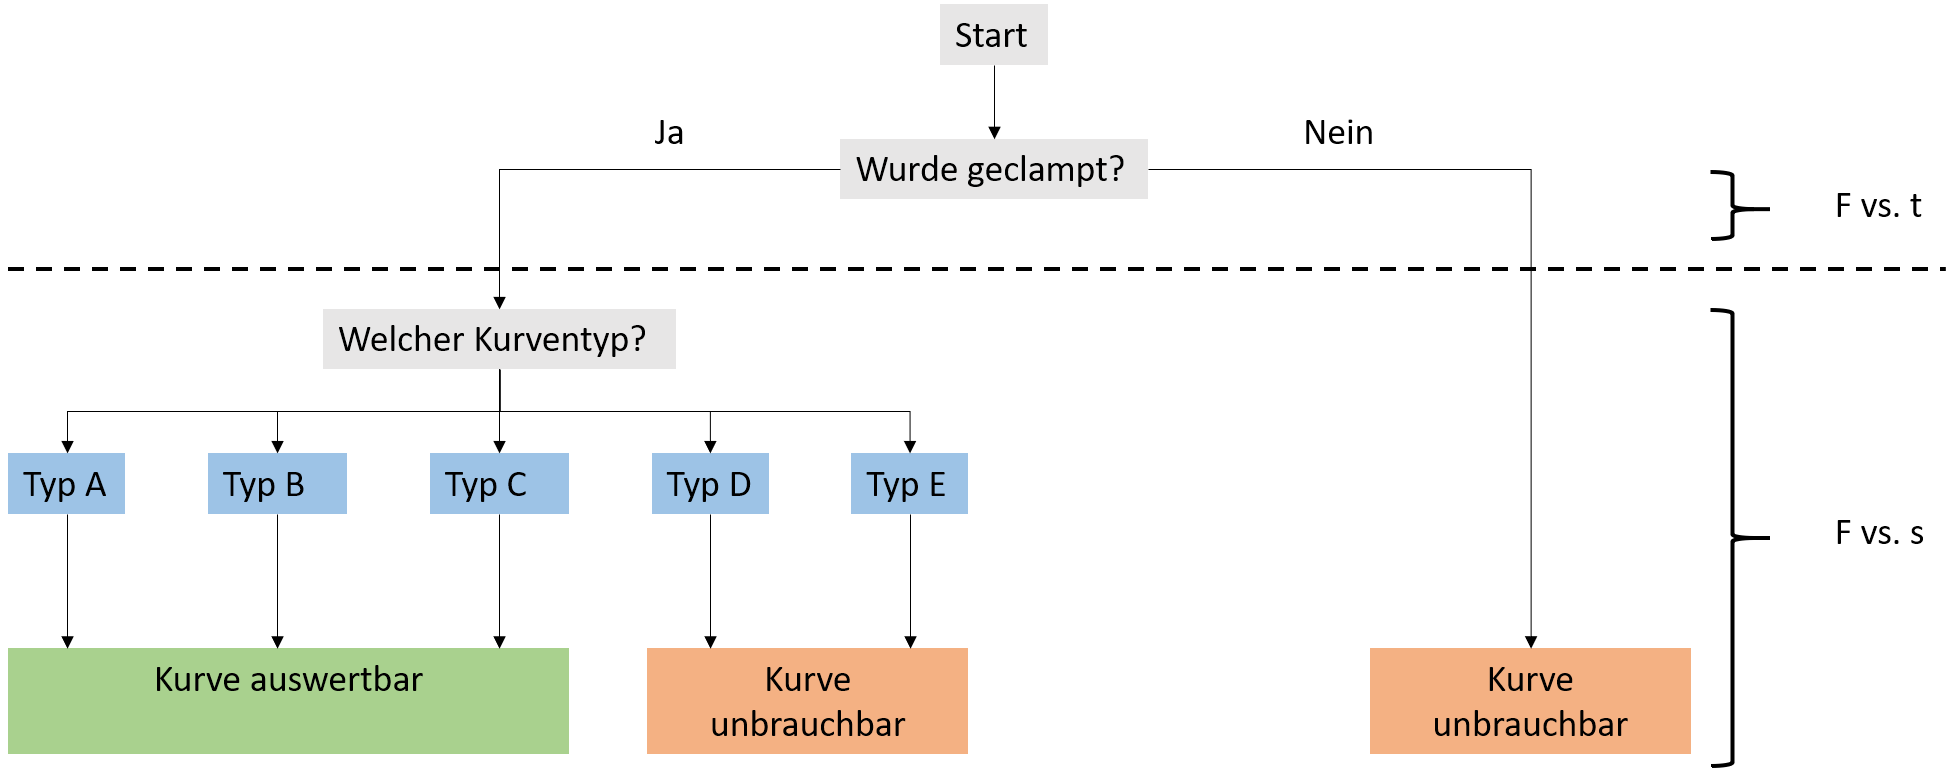
\includegraphics[width=\linewidth]{Abbildungen/Auswertung_ueberblick_VI.png}
	} % scalebox
	\caption[Ablaufschema der Kategorisierung]{Ablauf der Kategorisierung. Auswertbare Kraftkurven (Kategorie A und B) durften zusätzlich nicht bis zur maximalen Clampzeit gehalten werden oder einen Doppelpeak aufweisen. Die Kategorisierung erfolgte in zwei Schritten. Zunächst wurde anhand der Kraft-Zeit-Kurve (F vs. t) bestimmt ob ein Clampereigniss stattfand. Danach wurden die Kraftkurven in der Kraft-Abstand Darstellung (F vs. s) in die jeweiligen Kategorien eingeteilt.}
	\label{fig:kategorisierung}
	
\end{figure}

\subsubsection{Kategorie A}
\label{subsubsec:kategorie_a}

Kraftkurven dieser Kategorie wiesen während der gesamten Wegfahrkurve einen einzelnen Abriss auf. Dieser galt als Einzelmolekülinteraktion, wenn das für \ac{CMA} typische Plateau bei $300-400~pN$ zu erkennen war. In \abb~\ref{fig:kategoire_a_kurve} ist eine Kategorie A Kraftkurve dargestellt. Kurven aus dieser Kategorie konnten ohne weiteres in die Auswertung mit aufgenommen werden, da während des gesamten Experiments kein weiterer Abriss (insbesondere kürzere Abrisse) das Ereignis beeinflussten. In einigen Fällen kam es vor, dass bei besonders kurzen Abrissen ($< 300~nm$), kein Plateau sichtbar war. Solche Kurven wurden dennoch zur Kategorie A gezählt.

\begin{figure}[H]
	\centering
	\scalebox{\hscaleZero}{
		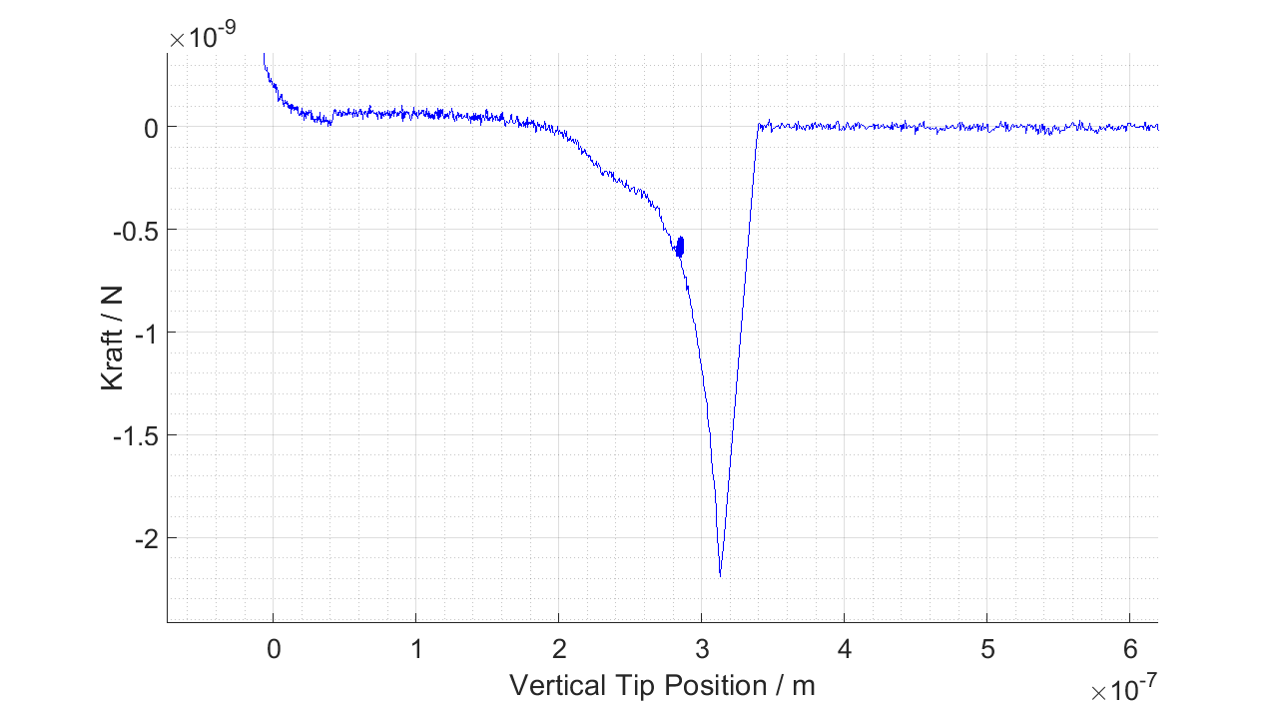
\includegraphics[width=\linewidth]{Abbildungen/Kategorien/A_I.png}
	} % scalebox
	\caption[Beispiel einer Kategorie A Kraftkurve]{Beispiel einer Kategorie A Kraftkurve. Diese Kurve zeigt das typische Plateau in einem Kraftbereich von 300 - 400 pN.}
	\label{fig:kategoire_a_kurve}
\end{figure}

\subsubsection{Kategorie B}
\label{subsubsec:kategorie_b}

Diese Kategorie wies in der Wegfahrkurve vor dem Hauptabriss (Peak bei der größten Abrisskraft) einen oder mehrere, vorgelagerte Abrisse bei einer Kraft von ca. $10-100~pN$ auf. Ein typisches Beispiel aus dieser Kategorie zeigt \abb~\ref{fig:kategorie_b_kurve}. Einzelmolekülinteraktionen aus dieser Kategorie konnten in vollem Umfang zur Auswertung herangezogen werden, sofern, die vorgelagerten Peaks vor, oder direkt am Beginn des Hauptabrisses lagen. Auch hier wurden, analog zu Kategorie A, kurze Abrisse ($< 300~nm$) zur Kategorie B gezählt.

\begin{figure}[H]
	\centering
	\scalebox{\hscaleZero}{
		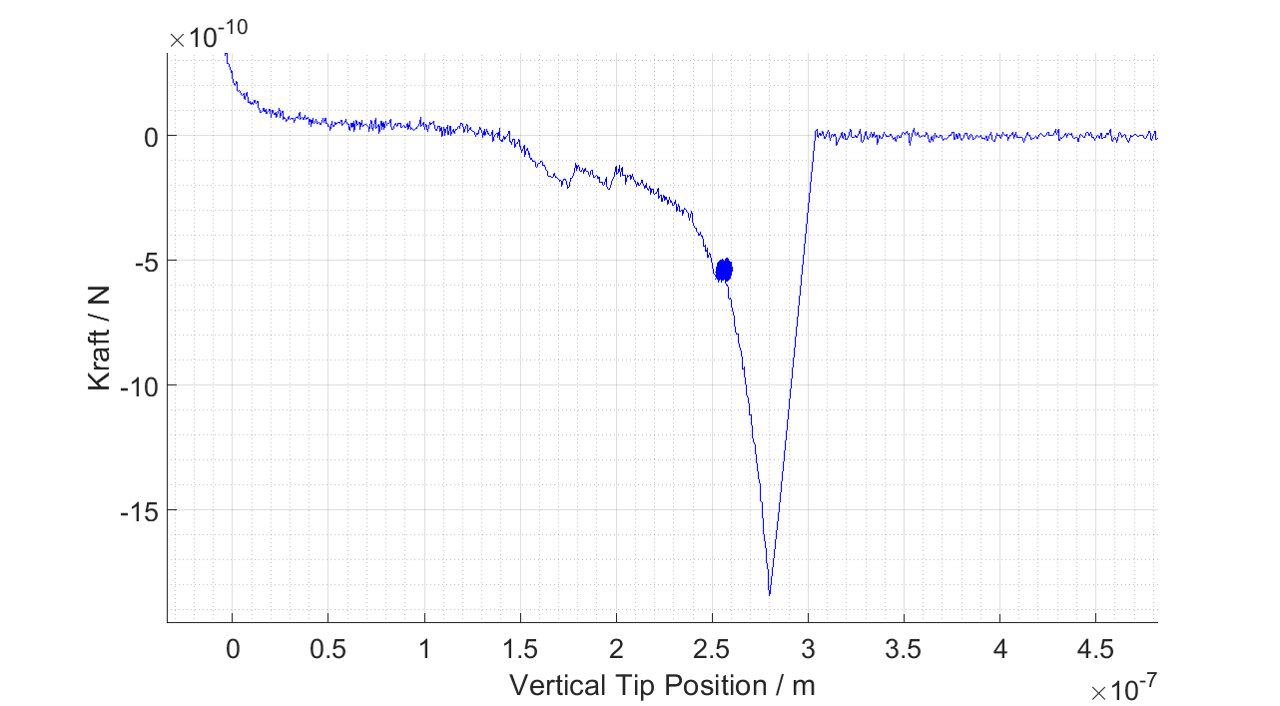
\includegraphics[width=\linewidth]{Abbildungen/Kategorien/BII.png}
	} % scalebox
	\caption[Beispiel einer Kategorie B Kraftkurve]{Beispiel einer Kategorie B Kraftkurve. Das typische Plateau von \acs*{CMA} bei 300 - 400 pN wird durch die, dem Hauptpeak vorgelagerten, kurzen Abrisse verdeckt. Die Vorgelagerten Abrisse liegen in der Größenordnung von 10 bis 100 pN.}
	\label{fig:kategorie_b_kurve}
\end{figure}

\subsubsection{Kategorie C}
\label{subsubsec:kategorie_c}

Dieser Kategorie wurden Kraftkurven zugeordnet, die in der Wegfahrkurve mehrere starke Abrisse (Abrisskraft lag im nN-Bereich) aufwiesen. Nicht alle Abrisse zeigten das \ac{CMA}-spezifische Plateau bei $300 - 400~pN$, starteten jedoch überwiegend von der gleichen Kraft. Das bedeutet, dass der Cantilever bis zu seiner Ausgangslage vor der Interaktion zurückkehrte und der nächste Abriss von der Nulllinie\footnote{Der Begriff Nulllinie wird im Abschnitt~\ref{subsec:auswertung_der_versuchsergebnisse} erläutert.} aus startete. Eine typische Kategorie C Kraftkurve zeigt \abb~\ref{fig:kategorie_c_kurve}. Kurven aus dieser Kategorie konnten nicht ausgewertet werden.

\begin{figure}[H]
	\centering
	\scalebox{\hscaleZero}{
		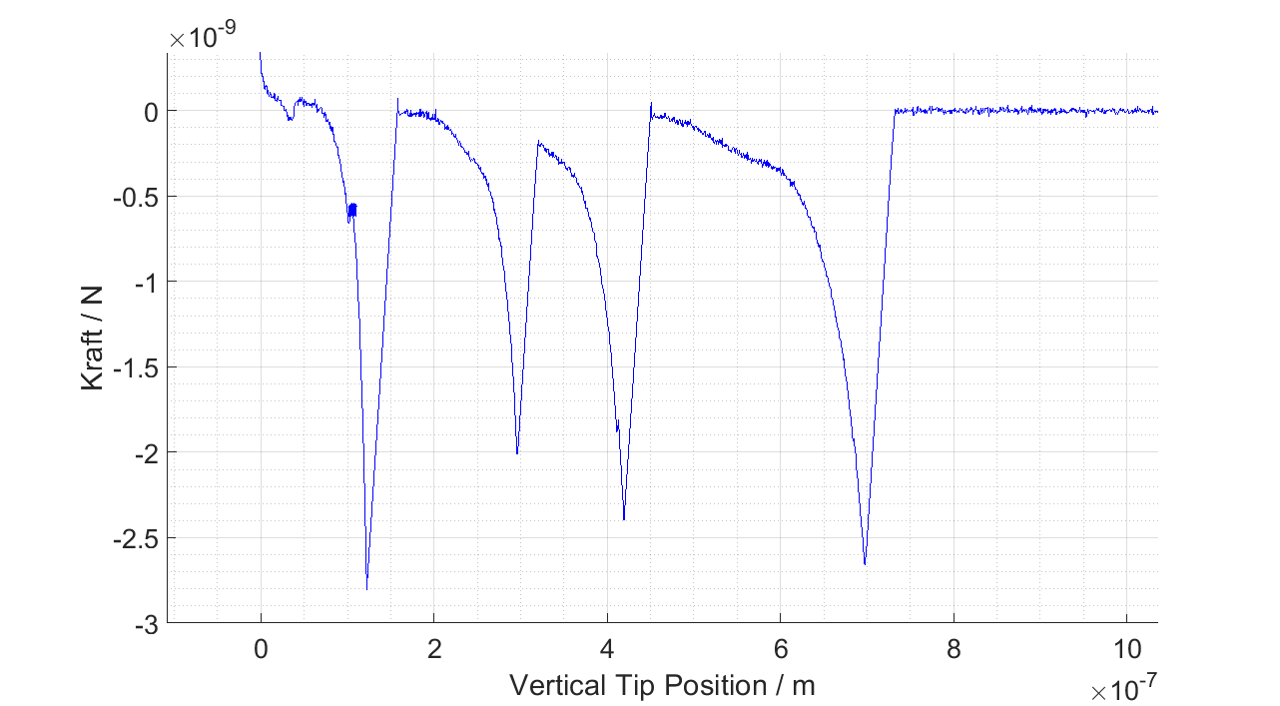
\includegraphics[width=\linewidth]{Abbildungen/Kategorien/CIII.png}
	} % scalebox
	\caption[Beispiel einer Kategorie C Kraftkurve]{Beispiel einer Kategorie C Kraftkurve. Alle aufeinander folgenden Abrisse beginnen in etwa bei der Nulllinie.}
	\label{fig:kategorie_c_kurve}
\end{figure}

\subsubsection{Kategorie D}
\label{subsubsec:kategorie_d}

Die Kurven aus dieser Kategorie wiesen in der Wegfahrkurve mehrere, überlagerte Abrisse auf. Typischerweise zeigten alle nachfolgenden Abrisse kein Plateau bei $300 - 400~pN$ und starteten bei höheren Kräften als der erste Abriss. Der Cantilever konnte zwischen den einzelnen Interaktionen nicht in seine Ausgangslage zurückkehren, sodass jeder weitere Abriss bei einer stärkeren Vorspannung auftreten musste. Ein typisches Beispiel einer Kategorie D Kraftkurve zeigt \abb~\ref{fig:kategorie_d_kurve}.

\begin{figure}[H]
	\centering
	\scalebox{\hscaleZero}{
		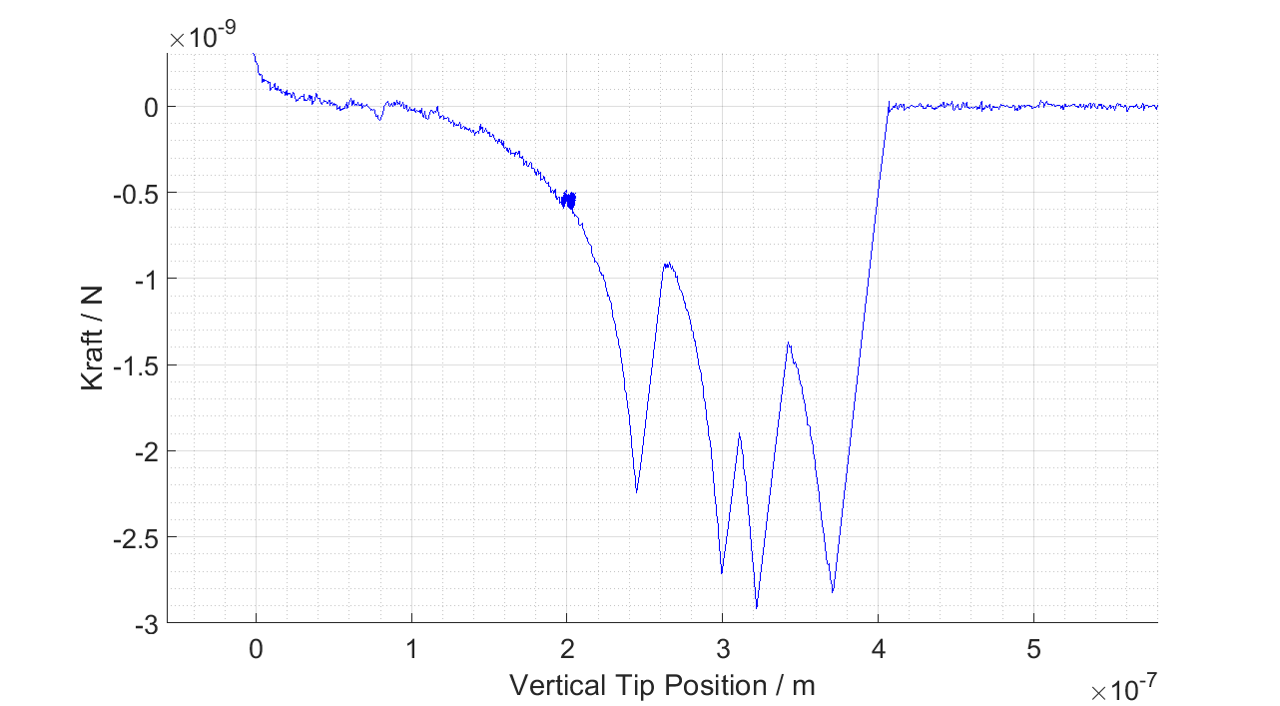
\includegraphics[width=\linewidth]{Abbildungen/Kategorien/DII.png}
	} % scalebox
	\caption[Beispiel einer Kategorie D Kraftkurve]{Beispiel einer Kategorie D Kraftkurve. Aufeinanderfolgende Abrisse starten bei einer höhere Kraft als die vorherigen Abriss. Es ist kein Plateau bei 300 - 400 pN zu erkennen.}
	\label{fig:kategorie_d_kurve}
\end{figure}

\subsubsection{Kategorie E}
\label{subsubsec:kategorie_e}

Diese Kategorie umfasst alle Kurven, welche nicht in eine der oberen Kategorien eingeordnet werden konnten. Typischerweise betraf das Kraftkurven mit ausschließlich unspezifischen Wechselwirkungen, wie beispielhaft in \abb~\ref{fig:kategorie_e_kurve} gezeigt wird.

\begin{figure}[H]
	\centering
	\scalebox{\hscaleZero}{
		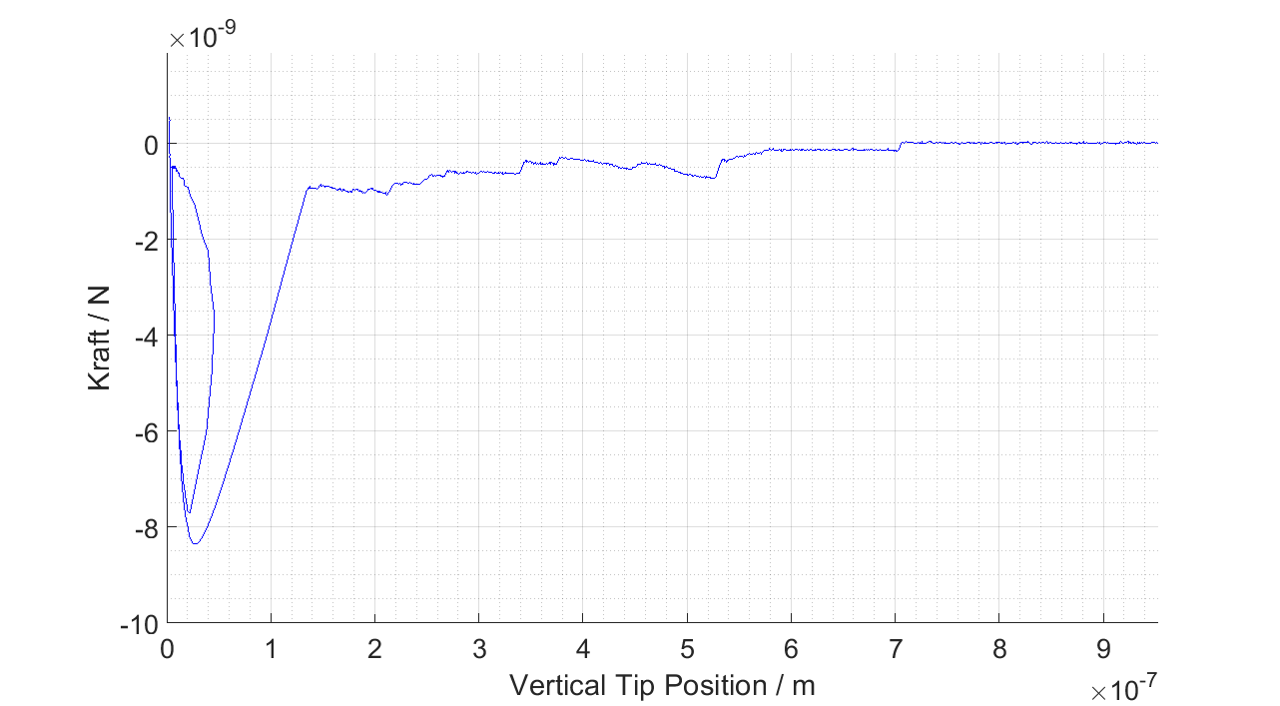
\includegraphics[width=\linewidth]{Abbildungen/Kategorien/EI.png}
	} % scalebox
	\caption[Beispiel einer Kategorie E Kraftkurve]{Beispiel einer Kategorie E Kraftkurve. Kraftkurve aus dieser Kategorie wiesen keine Merkmale auf, die eindeutig einer Einzelmolekülinteraktion mit \acs*{CMA} zuzuordnen waren.}
	\label{fig:kategorie_e_kurve}
\end{figure}

\subsubsection{Bemerkungen zu den Kraftkurven}
\label{subsubsec:bemerkungen_zu_den_kraftkurven}

Neben den eindeutig kategorisierbaren Details gab es Merkmale, welche in allen Kraftkurven auftreten konnten. Diese Merkmale beeinflussten nicht die Einordnung der Kraftkurven in die verschiedenen Kategorien (A bis E) und wurden während der Auswertung als Bemerkung zu jenen Messungen hinzugefügt.

\paragraph{Doppelpeak}
\label{par:doppelpeak}

Doppelpeaks gehörten prinzipiell zu Kraftkurven der Kategorie C, mit dem Unterschied, dass zwei direkt aufeinander folgende Peaks am Ende eines Abrisses sichtbar waren, wie in \abb~\ref{fig:doppelpeak} dargestellt. Doppelpeaks entstanden, wenn ein \ac{CMA}-Polymer unter Bildung einer Schlaufe (mehr als sechs Monomereinheiten) mehrfach an das Substrat oder die \spitze~gebunden haben. Den entsprechenden Kraftkurven wurde das Kürzel \ac{DP} hinzugefügt und wurden in der Auswertung ebenfalls nicht berücksichtigt.

\begin{figure}[H]
	\centering
	\scalebox{\hscaleZero}{
		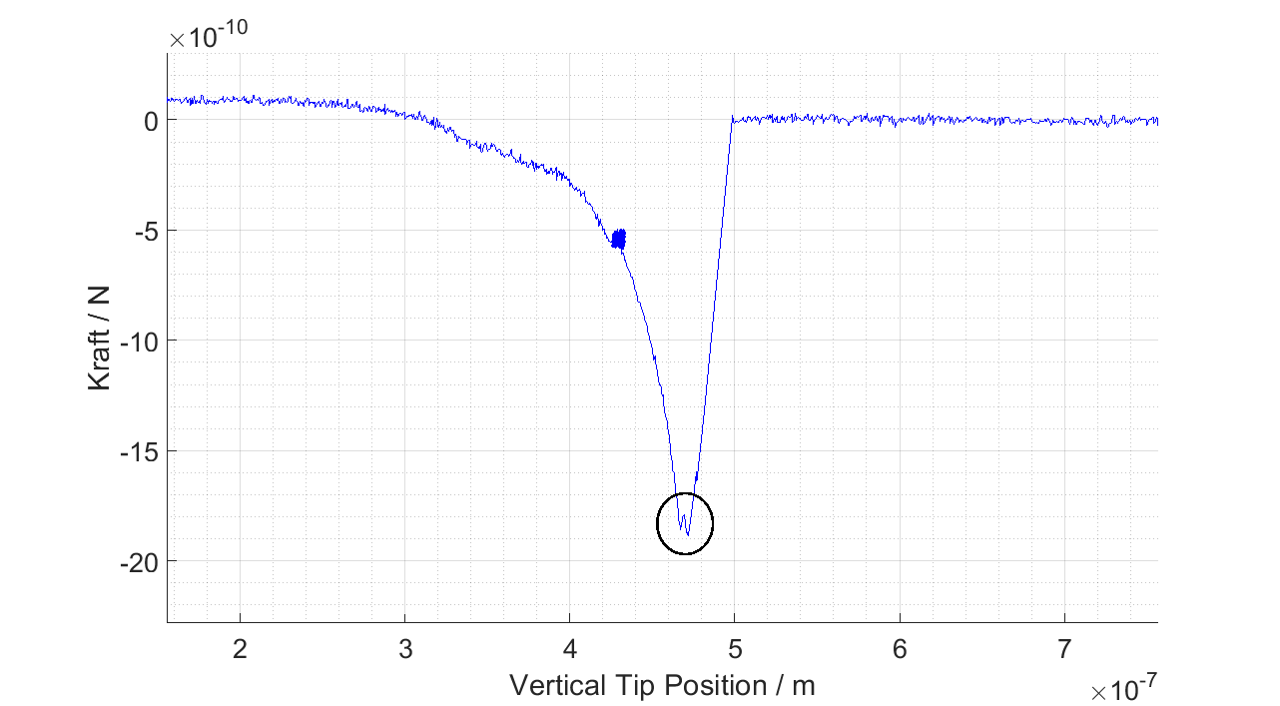
\includegraphics[width=\linewidth]{Abbildungen/Kategorien/DPII.png}
	} % scalebox
	\caption[Beispiel einer Kraftkurve mit Doppelpeak]{Beispiel einer Kraftkurve mit Doppelpeak.}
	\label{fig:doppelpeak}
\end{figure}

\paragraph{Maximale Clampzeit}
\label{par:maximale_clampzeit}

Es kam vor, dass einige Kurven bis zur maximal möglichen Clampzeit bei $800~pN$ gehalten werden konnten. Die Bindung wurde erst im 6. Segment der Force-Clamp-Experimente gebrochen. Kraftkurven mit dieser Besonderheit wurde das Kürzel \ac{tmax} hinzugefügt. Kraftkurven mit diesem Kürzel konnten nicht ausgewertet werden.

\subsection{Auswertung der Versuchsergebnisse}
\label{subsec:auswertung_der_versuchsergebnisse}

Die Messung der Abrisszeiten der aufgenommenen Kraftkurven wurde hauptsächlich mit der Data Processing Software von JPK durchgeführt. Für das Erstellen von \abbn~der Kraftkurven wurde ein eigens geschriebenes MATLAB-Skript verwendet. Für die Bestimmung der Geschwindigkeitskonstanten sowie die halblogarithmische Darstellung der Bindungsanzahl gegen die Zeit wurde Igor Pro 5 verwendet.\\
Zunächst wurde in Data Processing Korrekturen für die Nulllinie, für den Kontaktpunkt und der Cantileverauslenkung durchgeführt. Die Nulllinie ist die Cantileverauslenkung, die nicht vom Strecken des \spacers~stammt. dieser Offset in y-Richtung der Kraft-Abstand-Kurve wurde in Data Processing durch Mittelung des thermischen Rauschens anhand der ersten $10~\%$ der Hinfahrkurve bestimmt und von den y-Werten der gesamten Kraftkurve abgezogen. Der Kontaktpunkt repräsentiert den Punkt auf der Kraftkurve, der für den Kontakt der \spitze~mit dem Substrat steht. Durch die Stokes-Reibung liegen Hin- und Rückfahrkurve nicht direkt übereinander. Daher ist der Kontaktpunkt für das 1.Segment und das 3. Segment der Kraft-Abstand-Kurven auf der x-Achse gegeneinander verschoben. Der Kontaktpunkt für die Force-Clamp/ Ramp-Experimente wird als Schnittpunkt des 3. Segments mit der Nulllinie definiert und der Offset von allen x-Werten der Kraft-Abstand-Kurve abgezogen. Wird ein \spacer~zwischen  Substrat und \spitze~gestreckt, ist die gemessene z-Position um den Betrag der Cantileverauslenkung - bedingt durch das Strecken des \spacers~- zu lang. Die Korrektur dieser Auslenkung wird durch die Data Processing Software automatisch durchgeführt. Die, um die Cantileverauslenkung bereinigte z-Position, wird als \textit{vertical tip position} bezeichnet.\\
Anschließend wurden alle Kraftkurven kategorisiert. Während der Auswertung wurden die Lebensdauern $t$ aller Kraftkurven der Kategorie A und B ohne zusätzliche Bemerkung ermittelt. Die Ermittlung von $t$ geschah über den Step-Fit-Algorithmus der Data Processing Software und wurde über das gesamte 5. Segment der Kraft-Zeit-Kurven angewendet.\\
Nach der Auswertung der Kraftkurven erfolgte die Bestimmung von $k$ bzw. $\tau$. Dazu wurde Die Anzahl intakter Amidbindungen gegenüber $t$ aufgetragen. Danach konnte $k$ über einen biexponentiellen Zerfall ermittelt werden.

